\begin{filecontents*}{\jobname.xmpdata}
  \Title{sample}
\end{filecontents*}

\documentclass[b5paper,10.5pt,titlepage,openany]{ltjsbook}
\usepackage{graphicx}
\usepackage[pdfbox]{gentombow}
\usepackage[x-1a]{pdfx}

\usepackage{url}
\usepackage{listings}
\usepackage{bm}
\usepackage{amsmath}
\let\maketitle\relax
\usepackage{mytitle}

\usepackage{titlesec}
\lstset{
  backgroundcolor={\color[gray]{.95}},
  basicstyle={\small\ttfamily},
  lineskip=0truemm,
}

\renewcommand{\lstlistingname}{リスト}
\renewcommand{\figurename}{図}
% \renewcommand{\baselinestretch}{0.95}

\usepackage{luatexja-fontspec}
% https://fonts.google.com/specimen/Noto+Sans+JP
\setsansfont[
   UprightFont = *-Regular,
   BoldFont = *-Bold
 ]{NotoSansJP}
 \setsansjfont[
   UprightFont = *-Regular,
   BoldFont = *-Bold
 ]{NotoSansJP}

% ページの左右余白比の調整
\setlength{\marginparwidth}{0pt}
\setlength{\marginparsep}{0pt}
\setlength{\oddsidemargin}{0pt}
\setlength{\evensidemargin}{0pt}

% \setlength\intextsep{2truemm}
% \setlength\abovecaptionskip{1truemm}

\makeatletter
\renewcommand{\title}[1]{\gdef\@title{\bfseries\sffamily\gtfamily{#1}}}
\renewcommand{\author}[1]{\gdef\@author{\bfseries\sffamily\gtfamily{#1}}}
\renewcommand{\date}[1]{\gdef\@date{\bfseries\sffamily\gtfamily{#1}}}
\makeatother

\title{Sample document}
\author{daiiz\thanks{Twitter: \tt{@daizplus}, Scrapbox: \url{https://scrapbox.io/daiiz}}}
\date{2019冬 初版}

\hypersetup{final}

\begin{document}
\maketitle

\part{テスト} % Scrapbox page title line"
\label{textBlock-443b76e4bceb48ea2bca52261a1da542}
\chapter{Title}
先のRFCのSection. 3に「File Structure」の説明があるのでこれを読み、整理するとだいたい次のようになります。
\begin{itemize}
  \item 111
  \begin{itemize}
    \item 222
  \end{itemize}
  \item 111
  \begin{itemize}
    \item 222
    \begin{itemize}
      \item 333
      \item 333!
    \end{itemize}
    \item 2222
    \begin{itemize}
      \item 3333
      \item 3333
    \end{itemize}
  \end{itemize}
\end{itemize}

ふがー
\begin{itemize}
  \item 1111
  \item XML文書に対する描画スタイルを関する情報は、XSL (Extensible Stylesheet Language) という言語を用いて記述されます。スタイルシートというものの、CSSのように各要素に対する見た目を定義するものではなく、ソースとなるXMLツリーの任意のノードに着目してこれらに対する変換処理を書いていくため、テンプレート言語に近い存在です。
\end{itemize}

一般にXML文書は、専用のXSLTスタイルシートを適用することでSVGを含む他形式の文書に変換することができます。この処理はサーバー側とクライアント側の両方で行えるため、サーバーから配信されるスクリーンショット画像はXML形式とSVG形式のどちらでも選択可能となります。
オリジナルデータを参照しながら描画をカスタマイズしつつCustomElementなどで表示する場合はXMLデータを、img要素で直接表示したい場合はSVGデータを要求する、といった具合でクライアント側の都合に応じて使い分けられます。\\

\begin{figure}[h]
  \begin{center}
     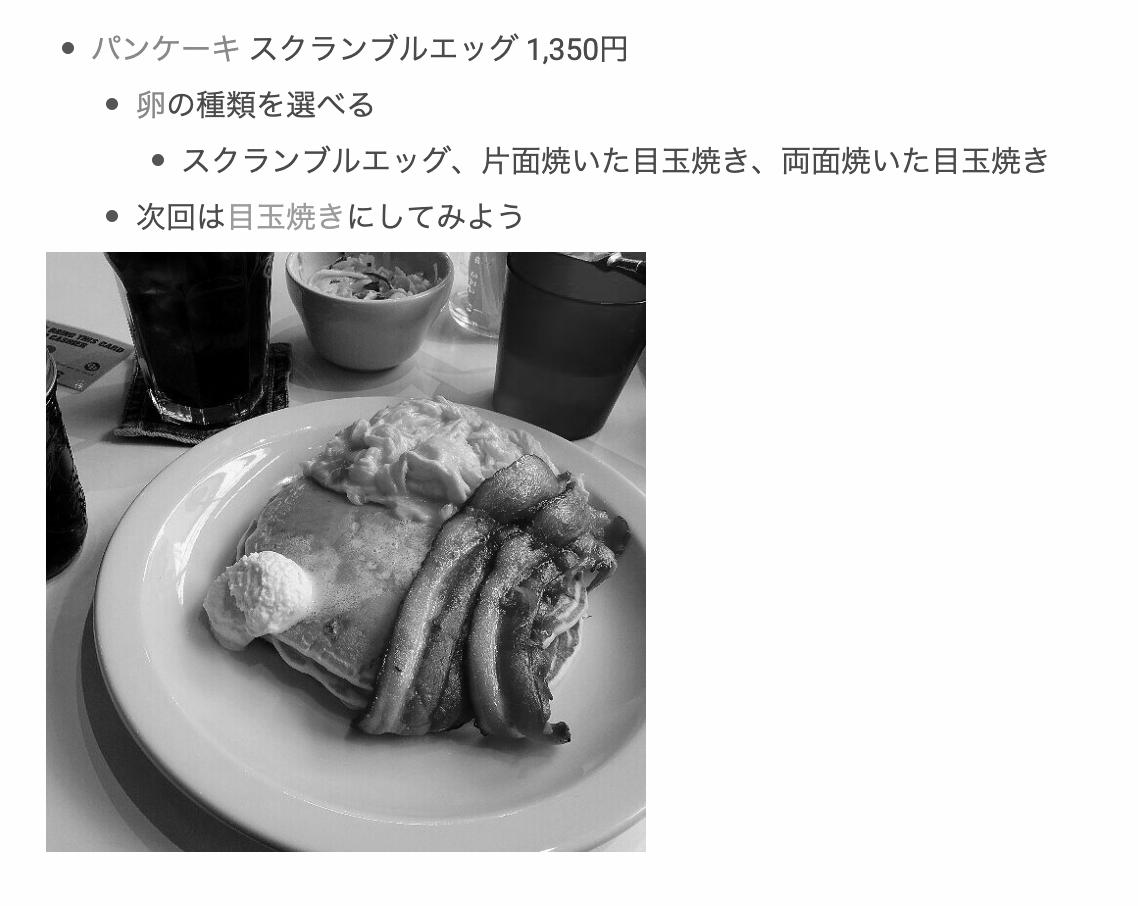
\includegraphics[width=0.7\linewidth]{./cmyk-gray-gyazo-images/retina_pancake.jpg}
     \caption{箇条書きの処理は結構大変}
     \label{xslt-story}
  \end{center}
\end{figure}
いい画像でしょ。『Implement Client-Hints HTTP header』(Firefox)\\

これはコードブロック
codeBlock

\end{document}
